
%Author : Senthilkumar Lakshmanan
%Email: senthilkumarl@live.com
\documentclass{article}
\usepackage[cmex10]{amsmath}
\usepackage{amsmath}
\usepackage{bm}
\usepackage{amsfonts}
\usepackage{tikz}
\usetikzlibrary{calc}
\usetikzlibrary{shapes.geometric, arrows}
\usetikzlibrary{shapes,fit} 
\tikzstyle{startstop} = [rectangle, rounded corners, minimum width=1.5cm, minimum height=0.5cm,text centered, draw=black, fill=red!30]
\tikzstyle{io} = [trapezium, trapezium left angle=70, trapezium right angle=110, minimum width=1.5cm, minimum height=0.5cm, text centered, draw=black, fill=blue!30, text width=4cm]
\tikzstyle{process} = [rectangle, minimum width=1.5cm, minimum height=0.5cm, text centered, draw=black, fill=orange!30, text width=4cm]
\tikzstyle{decision} = [diamond, minimum width=1.5cm, minimum height=0.5cm, text centered, draw=black, fill=green!30, text width=1.9cm, text height=0.3cm]
\tikzstyle{arrow} = [thick,->,>=stealth]

 
  \usetikzlibrary{external}
\tikzset{external/system call={latex \tikzexternalcheckshellescape -halt-on-error
-interaction=batchmode -jobname "\image" "\texsource" && 
dvips -o "\image".ps "\image".dvi &&
ps2eps "\image.ps"}}
\tikzexternalize[shell escape=-enable-write18]
			
\usepackage{pgfplots}


\begin{document}

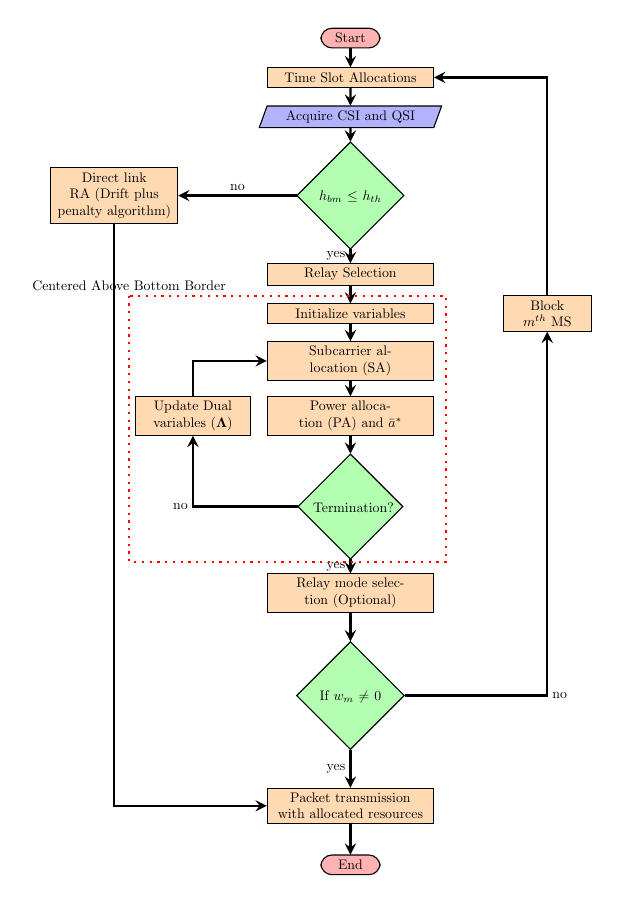
\begin{tikzpicture}[node distance=1cm, scale=0.5, transform shape]
[auto,
 block/.style ={rectangle, draw=blue, thick, fill=blue!20, text width=8cm,align=center, rounded corners, minimum height=8cm},
 line/.style ={draw, thick, -latex',shorten >=2pt},
 cloud/.style ={draw=red, thick, ellipse,fill=red!20,
 minimum height=1em}]

\node (start) [startstop] {Start};
\node (timpros) [process, below of=start] {Time Slot Allocations};
\node (chpros) [io, below of=timpros] {Acquire CSI and QSI};
\node (bmdec) [decision, below of=chpros, yshift=-1cm] {$h_{bm} \leq h_{th}$};
\node (dirpros) [process, left of=bmdec, xshift=-5cm, text width=3cm] {Direct link RA (Drift plus penalty algorithm)};
\node (rselpros) [process, below of=bmdec, yshift=-1cm] {Relay Selection};
\node (initpros) [process, below of=rselpros] {Initialize variables};
\node (blkpros) [process, right of=initpros, text width=2cm, xshift=4cm] {Block $m^{th}$ MS};
\node (satpros) [process, below of=initpros, yshift=-0.2cm] {Subcarrier allocation (SA)};
\node (patpros) [process, below of=satpros, yshift=-0.4cm] {Power allocation (PA) and $\bar{a}^*$};
\node (updtpros) [process, left of=patpros, xshift=-3cm, text width=2.7cm] {Update Dual variables ($\bm{\Lambda}$)};

\node (termdec) [decision, below of=patpros, yshift=-1.3cm] {Termination?};
\node (rmpros) [process, below of=termdec, yshift=-1.2cm] {Relay mode selection (Optional)};
\node (wmdec) [decision, below of=rmpros, yshift=-1.6cm] {If $w_m\neq 0$};
\node (pktpros) [process, below of=wmdec, yshift=-1.8cm] {Packet transmission with allocated resources};
\node (stop) [startstop,, below of=pktpros, yshift=-0.5cm] {End};
\draw [arrow] (start) -- (timpros);
\draw [arrow] (timpros) -- (chpros);
\draw [arrow] (chpros) -- (bmdec);
\draw [arrow] (bmdec) -- node[anchor=south] {no} (dirpros);
\draw [arrow] (bmdec) -- node[anchor=east] {yes} (rselpros);
\draw [arrow] (rselpros) -- (initpros);
\draw [arrow] (initpros) -- (satpros);
\draw [arrow] (satpros) -- (patpros);
\draw [arrow] (patpros) -- (termdec);
\draw [arrow] (rmpros) -- (wmdec);
\draw [arrow] (termdec) -| node[anchor=east] {no} (updtpros);
\draw [arrow] (updtpros) |- (satpros);
\draw [arrow] (termdec) -- node[anchor=east] {yes}(rmpros);
\draw [arrow] (wmdec) -- node[anchor=east] {yes}(pktpros);
\draw [arrow] (wmdec) -| node[anchor=west] {no}(blkpros);
\draw [arrow] (blkpros) |- (timpros);
\draw [arrow] (pktpros) -- (stop);
\draw [arrow] (dirpros) |- (pktpros);
%\node[draw=red, fit=(satpros) (patpros) (termdec) (updtpros), text width=8cm, text height=9cm](FIt1) {};
\draw[red,thick,dotted] ($(initpros.north west)+(-3.5,0.2)$)  rectangle ($(patpros.south east)+(0.3,-3.2)$);
\node [above] at ($(initpros.north west)+(-3.5,0.2)$) {Centered Above Bottom Border};
\end{tikzpicture}

\end{document}